\section{Ejercicio 2}

\subsection{Introducción}
\label{introej2}
	
\subsection{Explicación}

\paragraph{}
Primero, algunas definiciones:

\paragraph{}
\textbf{Def$_1$:}
\\
Un grafo $G$ es fuertemente orientable si existe una asignación de direcciones a los ejes del conjunto de ejes del grafo $G$ tal que el digrafo resultante es fuertemente conexo. 

\paragraph{}
\textbf{Def$_2$:}
\\
un puente, \textbf{arista de corte} o istmo es una arista que al eliminarse de un grafo incrementa el número de componentes conexos de éste. Equivalentemente, una arista es un puente si y sólo si no está contenido en ningún ciclo.

\paragraph{}
\textbf{Teorema} [Robbins, 1939] :\\
Un grafo conexo $G$ es fuertemente orientable si y solo si $G$ no tiene puentes (Demostración en el anexo).



\paragraph{} 
Con esté teorema podemos ver que si encontramos al menos 1 puente en nuestro grafo, significa que no podremos orientarlo como queremos, y de lo contrario, si encontramos que no hay ningun puente, podremos orientarlo. Por lo tanto, el algoritmo utilizado realiza exactamente esa comprobación. Veamos como trabaja:
 
\vspace*{3cm}

%segundo algoritmo:
\incmargin{1em}
\linesnumbered
\restylealgo{boxed}

\textbf{comprobación(Grafo G)}\\
\SetKw{Orden}{Complejidad:}
	\begin{algorithm}[H]
	\Orden{O($n^3$)}

    \textbf{var} eje : int $\leftarrow$ 0 \\
    \textbf{var} n : int $\leftarrow$ cantNodos(G) \\
				


     \While{eje $\leq$ m}{
      k $\leftarrow$ RecorridoSinEje(eje,G)\\

      \lIf{k $\neq$ n}{\textbf{return} no se puede} \\ eje $\leftarrow$ eje $+$ 1} \textbf{return} fuertemente conexo

  \end{algorithm}

RecorridoSinEje(eje,G) es una funcion que recorre el grafo $G$  (con BFS o DFS) sin utilizar la arista $eje$ y retorna la cantidad de nodos visitados, $k$. Como la forma de recorrer utilizada, solo recorre nodos conectados a la raiz (es decir, al nodo donde comienza el recorrido), quiere decir que el resultado k va a ser n (la cantidad total de nodos de $G$) si $G$ es conexo. De lo contrario, si k es menor que $n$, estamos en presencia de 2 componentes conexas (o más en el caso de $eje = 0$). Por lo tanto, el eje sacado, era un puente. 

\paragraph{}
\underline{Aclaración: }
\\
Cuando eje = 0, representa, recorrer a G completo con todos sus nodos. En este punto podria pasar que G no sea conexo y esta función devolvería el resultado correspondiente.


\subsection{Anexo: Demostraciones}
\label{demostraciones2}


\paragraph{}
\textbf{Teorema} [Robbins, 1939]:\\
Un grafo conexo $G$ es fuertemente orientable si y solo si $G$ no tiene puentes.


\paragraph{} 
\textbf{Demostración:} \underline{\textbf{$\rightarrow$)}}

Utilizando el contrareciproco, supongamos que el grafo $G$ tiene una arista de corte $e$ que une a los vertices $u$ y $v$. Entonces el unico camino entre $u$ y $v$  o $v$ y $u$ en el grafo $G$ es $e$ (ver figura). Por lo tanto para cualquier asignacion de direcciones, el nodo cola($e$) nunca va a poder ser alcanzada por el nodo cabeza($e$) (ver cuadro 1).

	\begin{table}[h!] %ubicacion de la tabla
		\centering %centra la tabla
			\begin{tabular}{c}
				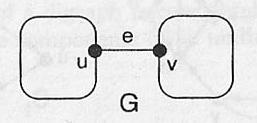
\includegraphics[scale=0.7]{./otros/figura1.jpg} 

				\end{tabular}
				\caption{} %titulo de la tabla
				\label{} %con esto puedo referenciar a la tabla \ref{Tiempo metodos}
	\end{table}

\paragraph{} 
\textbf{Demostración:} \underline{\textbf{$\leftarrow$)}}

Supongamos que $G$ es un nodo conexo sin aristas de corte. Por esto toda arista en $G$ cae en un circuito de $G$.
Para hacer que $G$ sea fuertemente orientable, empezaremos con cualquier circuito ($D_0$) de $G$ y dirigiremos sus ejes en una dirección (obteniendo un circuito dirigido). Si el ciclo $D_0$ contiene todos los nodos de $G$, entonces la orientación esta completa (ya que $D_0$ es fuertemente conexo). De lo contrario, hay que elegir cualquier eje $e$ uniendo a un vertice $u$ en $D_0$ y a un vertice $v$ en $V_G - V_{D_0}$ (ese eje existe ya que $G$ es conexo). Sea C = $\left\langle u,e,v,...,u  \right\rangle$ un ciclo que contiene al eje $e$, y sea $w$ el primer vertice luego de v en $C$ que cae en el ciclo $D_0$ (ver cuadro 2).

	\begin{table}[h!] %ubicacion de la tabla
		\centering %centra la tabla
			\begin{tabular}{c}
				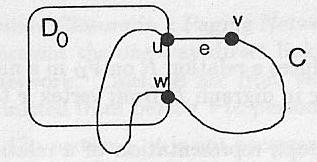
\includegraphics[scale=0.7]{./otros/figura2.jpg} 

				\end{tabular}
				\caption{} %titulo de la tabla
				\label{} %con esto puedo referenciar a la tabla \ref{Tiempo metodos}
	\end{table}

\paragraph{}
A continuación, direccionamos los ejes de este camino entre $v$ a $w$, obteniendo el camino dirigido $v-w$ que llamaremos $P$. Luego direccionamos el eje $e$ desde $u$ hasta $v$ y consideramos el digrafo $D_1$ que se forma agregando el eje dirigido $e$ a $D_0$ y todos los vertices y ejes dirigidos del camino $P$. Como $D_0$ es fuertemente conexo, entonces hay un camino dirigido de $w$ a $u$ ($Q$) en $D_0$ (ver cuadro 3). La concatenación de $P$ con $Q$ y el eje dirigido $e$ forman un circuito simple direccionado que contiene $u$ y los nuevos vertices de $D_1$. (si los vertices $u$ y $w$ son el mismo, entonces $P$ satiface ser un circuito simple dirigido)



\paragraph{}
Por lo tanto, el vertice $u$ y todos estos nuevos vetices son mutuamente alcanzables en $D_1$ y además $u$ y cada vectice del digrafo $D_0$ tambien son mutuamente alcanzables, y, por lo tanto , el digrafo $D_1$ es fuertemente conexo. Este proceso puede continuar hasta que el digrafo $D_1$ para algun $l$ $\geq$ 1, contenga todos los vertices de $G$. En este punto, cualquier asignacion de direcciones hacia las aristas sin direccion restantes completaran la orientación de $G$, puesto que contendrá el digrafo fuertemente conexo $D_l$ como subdigrafo.


%\clearpage

	\begin{table}[h!] %ubicacion de la tabla
		\centering %centra la tabla
			\begin{tabular}{c}
				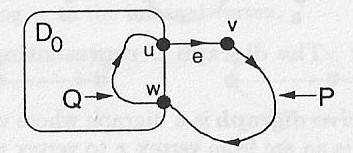
\includegraphics[scale=0.7]{./otros/figura3.jpg} 

				\end{tabular}
				\caption{} %titulo de la tabla
				\label{} %con esto puedo referenciar a la tabla \ref{Tiempo metodos}
	\end{table}

